\section{Formal Analysis}
\subsection{Alloy code}


\begin{lstlisting}[language=alloy]
    
 //Signatures

    abstract sig Bool {}
    one sig TRUE extends Bool {}
    one sig FALSE extends Bool {}

    abstract sig BatteryPolicy {}
    one sig Discharge extends BatteryPolicy {}
    one sig Disable extends BatteryPolicy {}
    one sig Recharge extends BatteryPolicy {}
    one sig Mantain extends BatteryPolicy {}

    abstract sig SocketType {}
    one sig Rapid extends SocketType {}
    one sig Fast extends SocketType {}
    one sig Slow extends SocketType {}    


    sig StationBattery{
        capacity: one Int,
        level: one Int
    }{
capacity >= 0
level >= 0}

    sig Socket{
        socketid: one Int,
        type: one SocketType,
        cost: one Int,
        isOccupied: one Bool,
        specialOffer: one Bool,
        percentageOffer: one Int

    }{      socketid > 0 
percentageOffer > 0
cost > 0
   } 
 
    sig ElectricVehicle{}

    abstract sig AccountRegistration {
    username: one Username,
    password: one Password,
    email: one Email
    }

    sig Email {}
    sig Username{}

    sig Password{}
    { //each password is associated to a registration (some registration may have the same password)
        all p: Password | (some r: AccountRegistration | r.password = p)
    }

sig Birthday{}
    sig Customer extends AccountRegistration{
	    electricvehicle: some ElectricVehicle,
	    birthday: one Birthday,
	    isActive: one Bool,
	booking: set Booking,
	suggestionbooking: lone SuggestionBooking

	
    }

    sig CPO extends AccountRegistration{
	name: one Name	,
	stations: some ChargingStation 
    }

    sig GPSPosition {}
    sig Name{}

    //We use a simplified model of a time
    sig Time {
	    time: one Int
    }{time >= 0}

    abstract sig BookingAbstract {
	 startTime: one Time,
	 endTime: one Time,
	socket: one Socket ,   
	station: one ChargingStation
    }
{startTime.time < endTime.time}

    sig ChargingStation{
        id: one Int,
        batterypolicy: one BatteryPolicy,
	location: one GPSPosition,
	socket: some Socket,
	battery: one StationBattery
    }{id > 0}
    
    sig Booking extends BookingAbstract {
	    id: one Int
   }
{id>0}
    
    sig SuggestionBooking extends BookingAbstract {}
   
    
    -----------------------------------------------------------------
    
    // Facts
    
  	fact{ //a unique username is associated to each registration    
		no disj r1, r2: AccountRegistration | r1.username = r2.username
    	}

   	fact{ //a unique email address is associated to each registration   
		no disj r1, r2: AccountRegistration | r1.email = r2.email
    	}

   	fact { //The CPO name must be unique          
		no disj c1, c2: CPO | c1.name = c2.name
    	}      

   	fact{  //each socket in the same charging station has a different id   
		all c: ChargingStation | (no disj s1, s2: Socket | s1.socketid = s2.socketid
		and (s1 in c.socket) and (s2 in c.socket))	
  	 }

	fact{ //all locations connected   
		all g: GPSPosition | one c: ChargingStation | g= c.location
	}
	
	fact{ //all bookings connected   
		all b: Booking | one c: Customer | b in c.booking
	}
	fact{ //all suggested bookings connected   
		all s: SuggestionBooking | one c: Customer | s = c.suggestionbooking
	}

	fact{ //all email connected   
		all e: Email | one a:  AccountRegistration | e= a.email
	}
	
	fact{ //each charging station has a different station battery 
		all c: ChargingStation | no disj s1, s2: StationBattery | c.battery = s1
		and c.battery = s2
	}

	fact { //Each ChargingStation has a unique CPO    
		all s: ChargingStation | no disj c1, c2: CPO | s in (c1.stations) and s in (c2.stations)
    	}  

	fact{ //all electric vehicle connected   
		all e: ElectricVehicle | one c: Customer | e in (c.electricvehicle)
	}	

	fact{ //all names connected   
		all n: Name | one c: CPO | n= c.name
	}

	fact{ //all sockets connected      
		all s: Socket | one c: ChargingStation | s in ( c.socket)
	}

	fact{ //all station batteries connected    
		all b: StationBattery | one c: ChargingStation | b= c.battery
		}

	fact{ //all usernames connected      
		all u: Username | one a:  AccountRegistration| u = a.username
	}

	fact{ //all birthdays connected      
			 all b: Birthday | some c: Customer | b = c.birthday
	}

	fact{ //all charging stations connected      
		all cs: ChargingStation | one c:  CPO| cs in c.stations
	}

    	fact{  //different Customers have a different set of electric vehicles   
    		no disj c1, c2 : Customer | c1.electricvehicle = c2.electricvehicle
    	}
	
	
	fact{  //the booked socket must be in the corresponding charging station   
    		all b: BookingAbstract |  ((b.socket) in (b.station.socket))
    	}
	
	

	fact{  // Cannot exist two bookings at the same time in the same socket
     		no disj b1, b2: Booking | b1.socket = b2.socket and b1.station= b2.station and 
		((b1.startTime.time > b2.startTime.time and b2.endTime.time > b1.endTime.time) 
		or (b2.startTime.time < b1.endTime.time) or
		(b2.endTime.time > b1.startTime.time) ) 
	
    	}


	fact{ //Customer can have just one booking at the time
     	 	all c: Customer | (no disj b1, b2: Booking| (b1 in c.booking and b2 in c.booking) and
		((b1.startTime.time > b2.startTime.time and b2.endTime.time > b1.endTime.time) 
		or (b2.startTime.time < b1.endTime.time and b2.endTime.time > b1.endTime.time ) or
		(b2.endTime.time > b1.startTime.time and b1.endTime.time > b2.endTime.time ) ) 

		and  b1.startTime.time = b2.startTime.time and b1.endTime.time = b2.endTime.time)
} //non funziona bene
			
    	
	fact{ //All bookings have a different id 
     	 	no disj b1, b2: Booking | b1.id = b2.id
	
    	}
	
	
//	fact{ //Customer doesn't have a suggested booking during a booking
     	 //	}
    

	

------------------------------------------------------------
//predicates

// simulation  that  shows  the  result  of some customer registrations
pred world1 {
	#Customer = 3
	#CPO = 0
	#Password > 1
	#Time = 0
	#ElectricVehicle > 2
	#SuggestionBooking = 0
	#Booking = 0
}
run world1 for 7

// simulation  that  shows  the  result  of some CPOs and the corresponding Charging Stations
pred world2 {
	#Customer = 0
	#CPO = 2
	#ChargingStation = 2
	#Time = 0
	#SuggestionBooking = 0
	#Booking = 0
	#Socket > 2
}
run world2 for 7

// simulation  that  shows  the  result  of some bookings and suggested bookings
pred world3 {
	#Customer = 1
	#ChargingStation = 2
	#Socket = 2
	#Booking  = 2
	#SuggestionBooking > 0
}
run world3 for 7







    
\end{lstlisting}
\newpage
\subsection{Worlds}
\begin{figure}[H]
	\hspace{-30pt}
	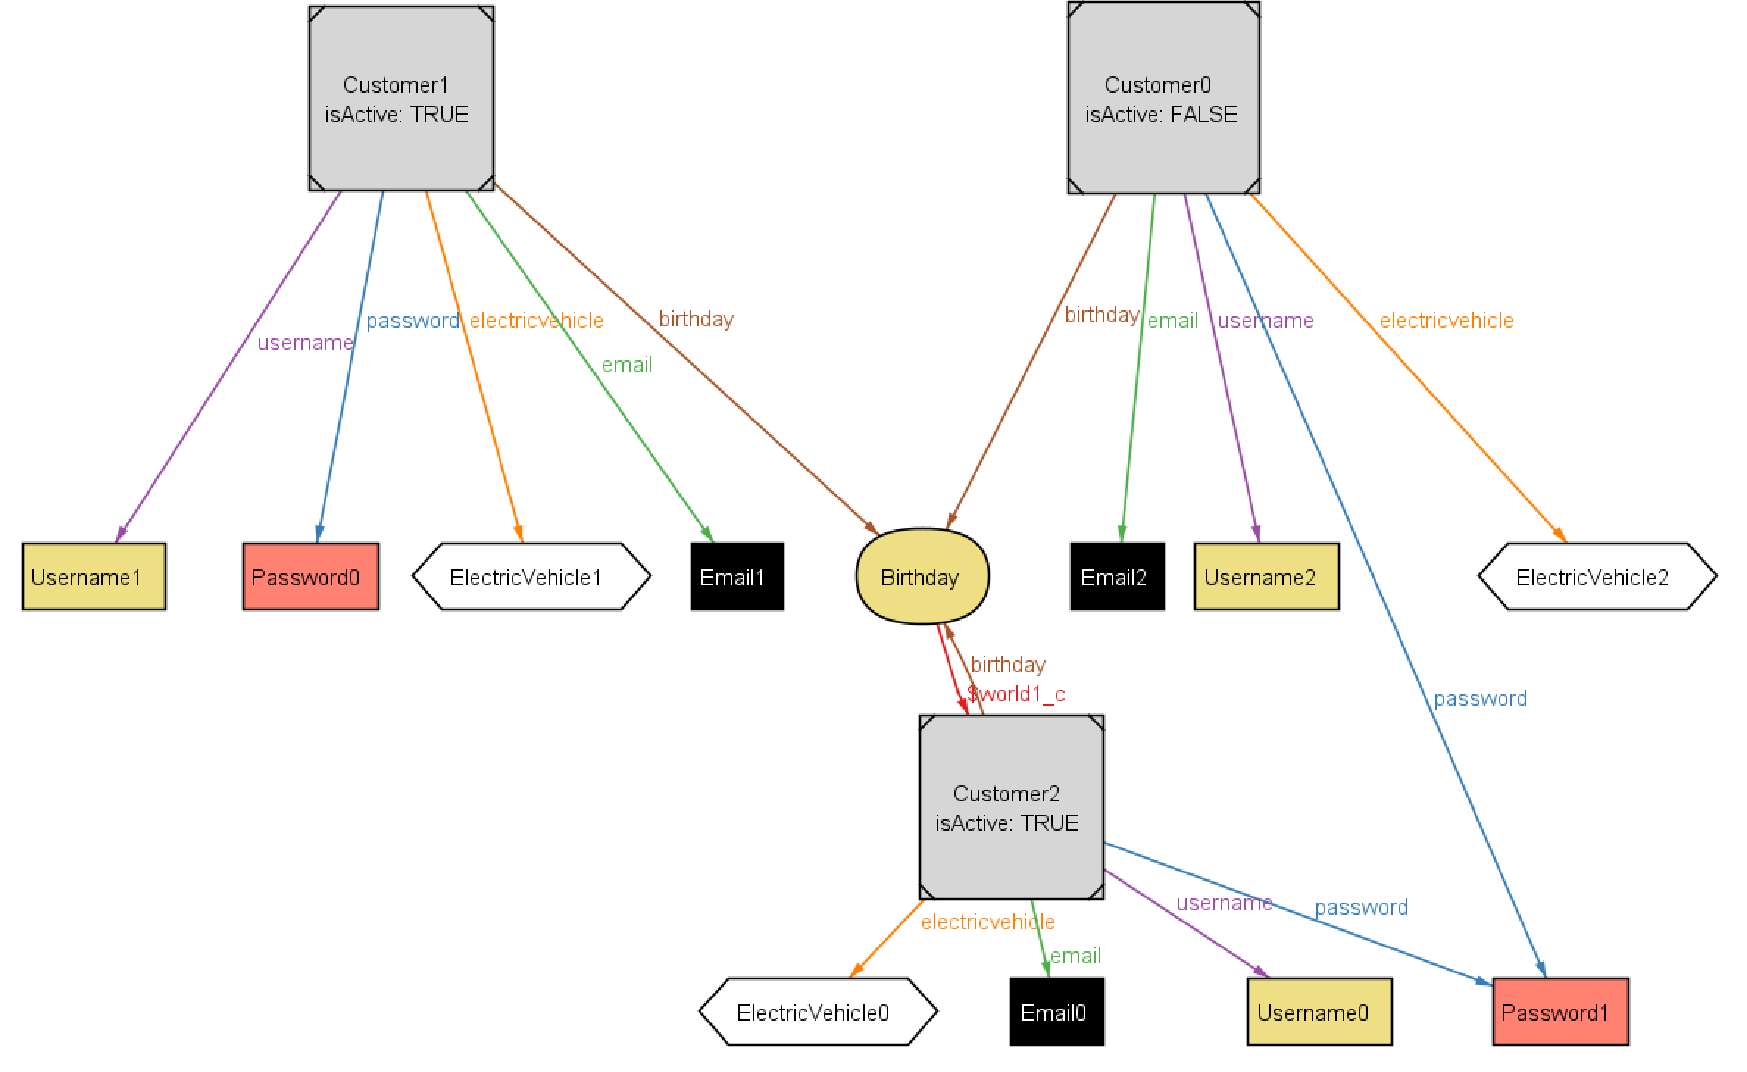
\includegraphics[width=1.2\textwidth]{img/world1.pdf}
	\caption{temp}
\end{figure}
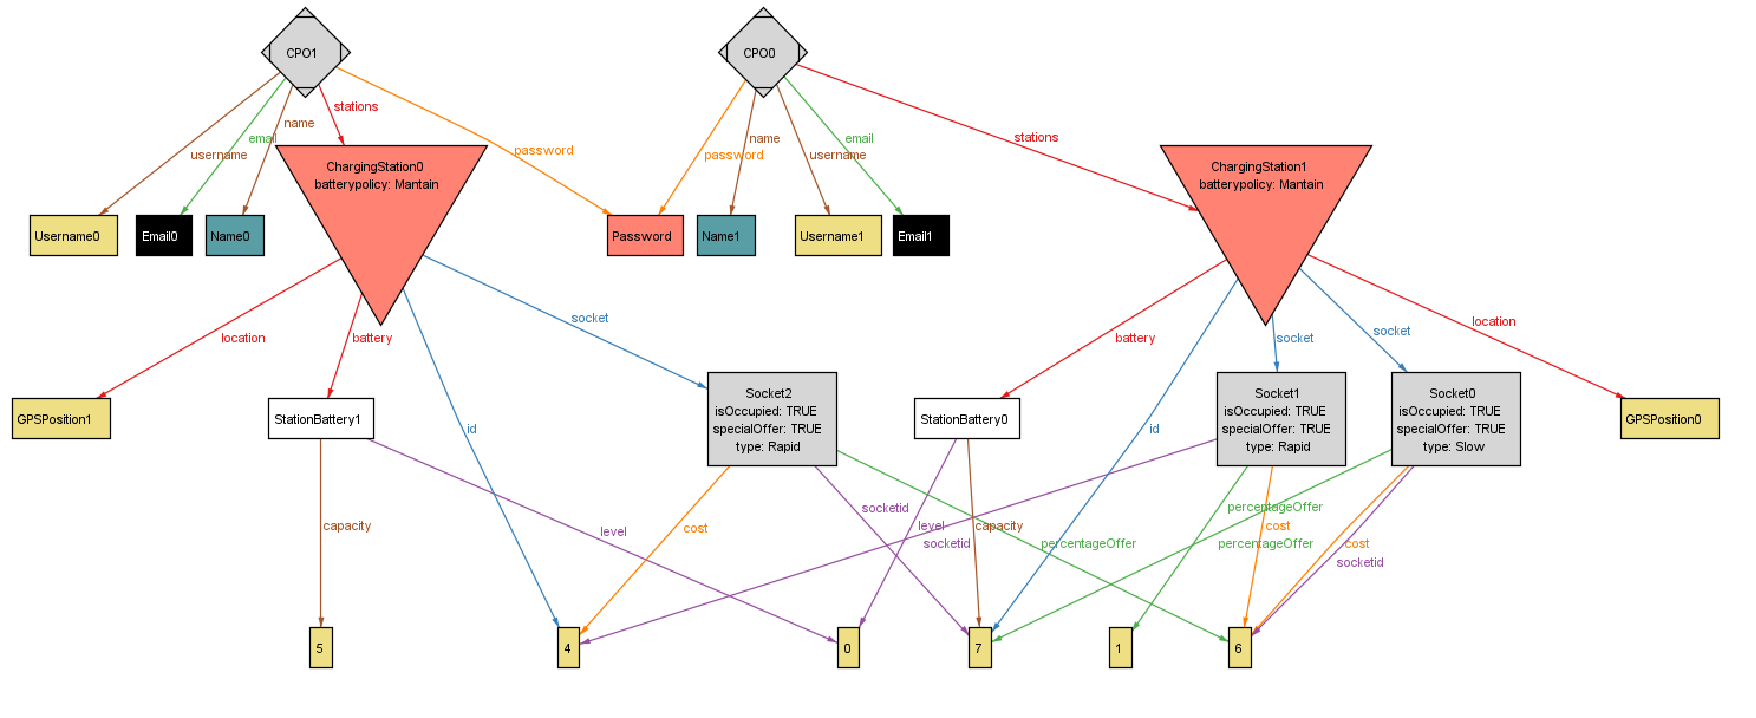
\includegraphics[width=1.2\textwidth]{img/world2.pdf}
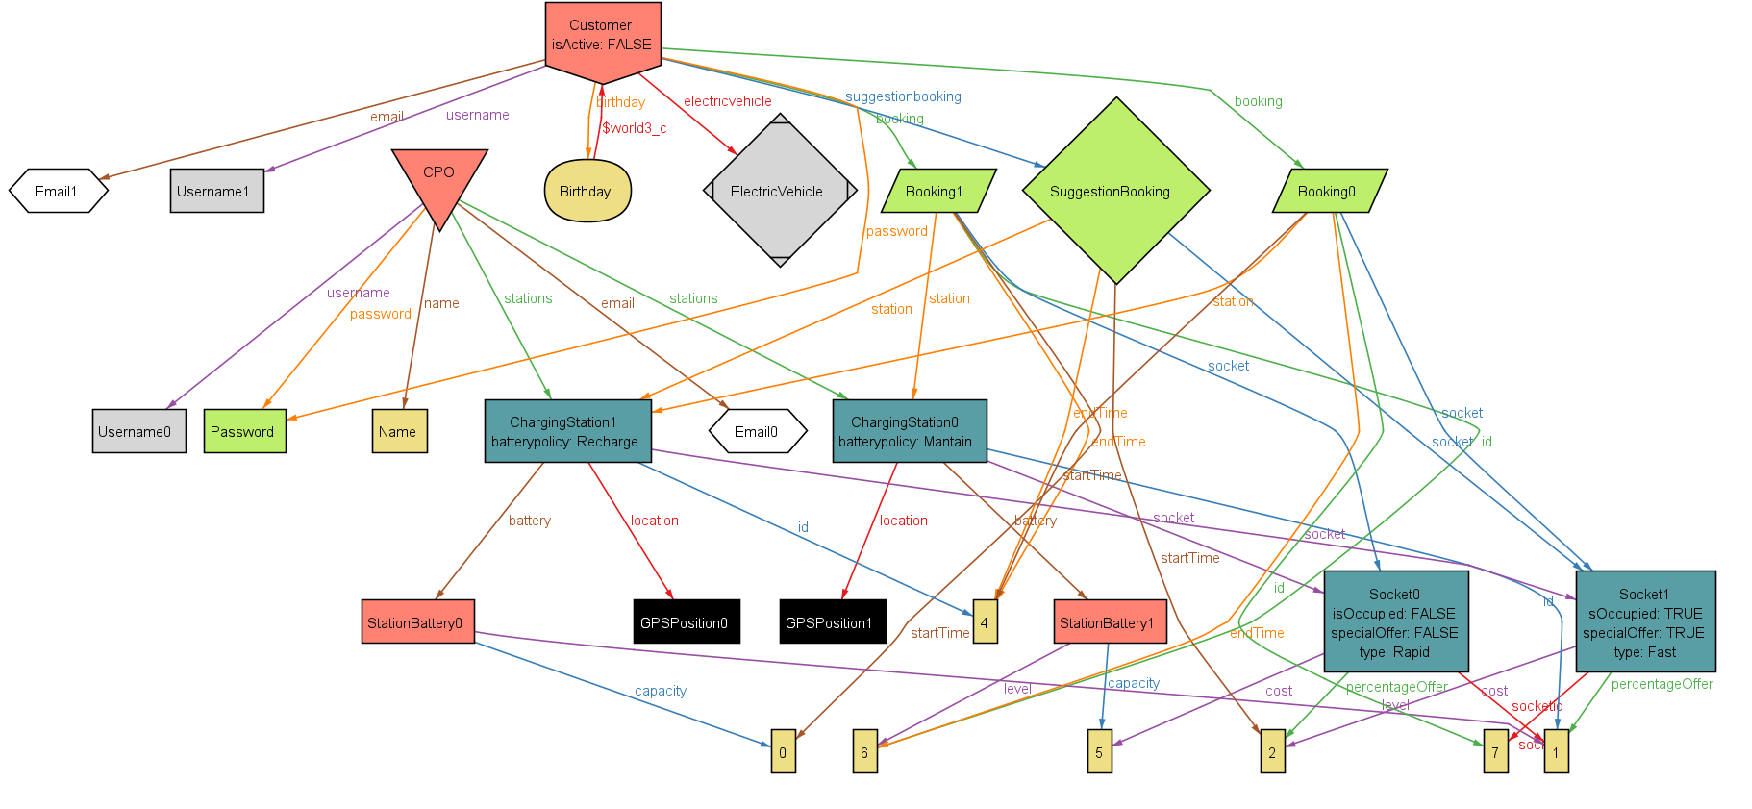
\includegraphics[width=1.2\textwidth]{img/world3.pdf}